% --- LaTeX CV Template - S. Venkatraman --- CURRICULUM VITAE

% Set document class and font size
\documentclass[letterpaper, 11pt]{article}
\usepackage[utf8]{inputenc}
\usepackage{wrapfig}

\usepackage[style=ieee, sorting=ydnt]{biblatex} % instead of bibtex; sorts them in reverse chronological order: ydnt
\addbibresource{Tex_publications_since2002.bib}


% Package imports
\usepackage{setspace, longtable, graphicx, hyphenat, hyperref, fancyhdr, ifthen, everypage, enumitem, amsmath, setspace}

% --- Page layout settings ---

% Set page margins
\usepackage[left=1in, right=1in, bottom=0.7in, top=0.7in]{geometry}

% Set line spacing
\renewcommand{\baselinestretch}{1.15}

% --- Page formatting ---

% Set link colors
\usepackage[dvipsnames]{xcolor}
\hypersetup{colorlinks=true, linkcolor=RoyalBlue, urlcolor=RoyalBlue}

% Set font to Libertine, including math support
\usepackage{libertine}
\usepackage[libertine]{newtxmath}

% Remove page numbering
\pagenumbering{gobble}

% --- Document starts here ---

\begin{document}

% Name and date of last update to this document
\noindent{\Huge{Li-Hsing Tex Chi, D.D.S., Ph.D.}
\hfill{\it\footnotesize Updated \today}}

% --- Contact information and other items ---

\vspace{0.5cm} 
\begin{center}
\begin{tabular}{lll}
% Line 1: Email, GitHub, office location
\textbf{Email}: d622101005@tmu.edu.tw      &
\hspace{0.2cm} \textbf{GitHub}: /github.com/texchi2    &
\hspace{0.2cm} 	\textbf{Office}: TMWH \\

% Line 2: Phone number, LinkedIn, citizenship
\textbf{Phone}: +886 970746852   & 
\hspace{0.2cm} \textbf{ResearchGate}: 
/profile/Li\_Hsing\_Chi &
%LinkedIn: /in/tex-chi-073523/   & 
\hspace{0.2cm} \textbf{Citizenship}: Taiwan 
\end{tabular}
\end{center}

\begin{wrapfigure}{r}{0.3\textwidth}
    \centering
    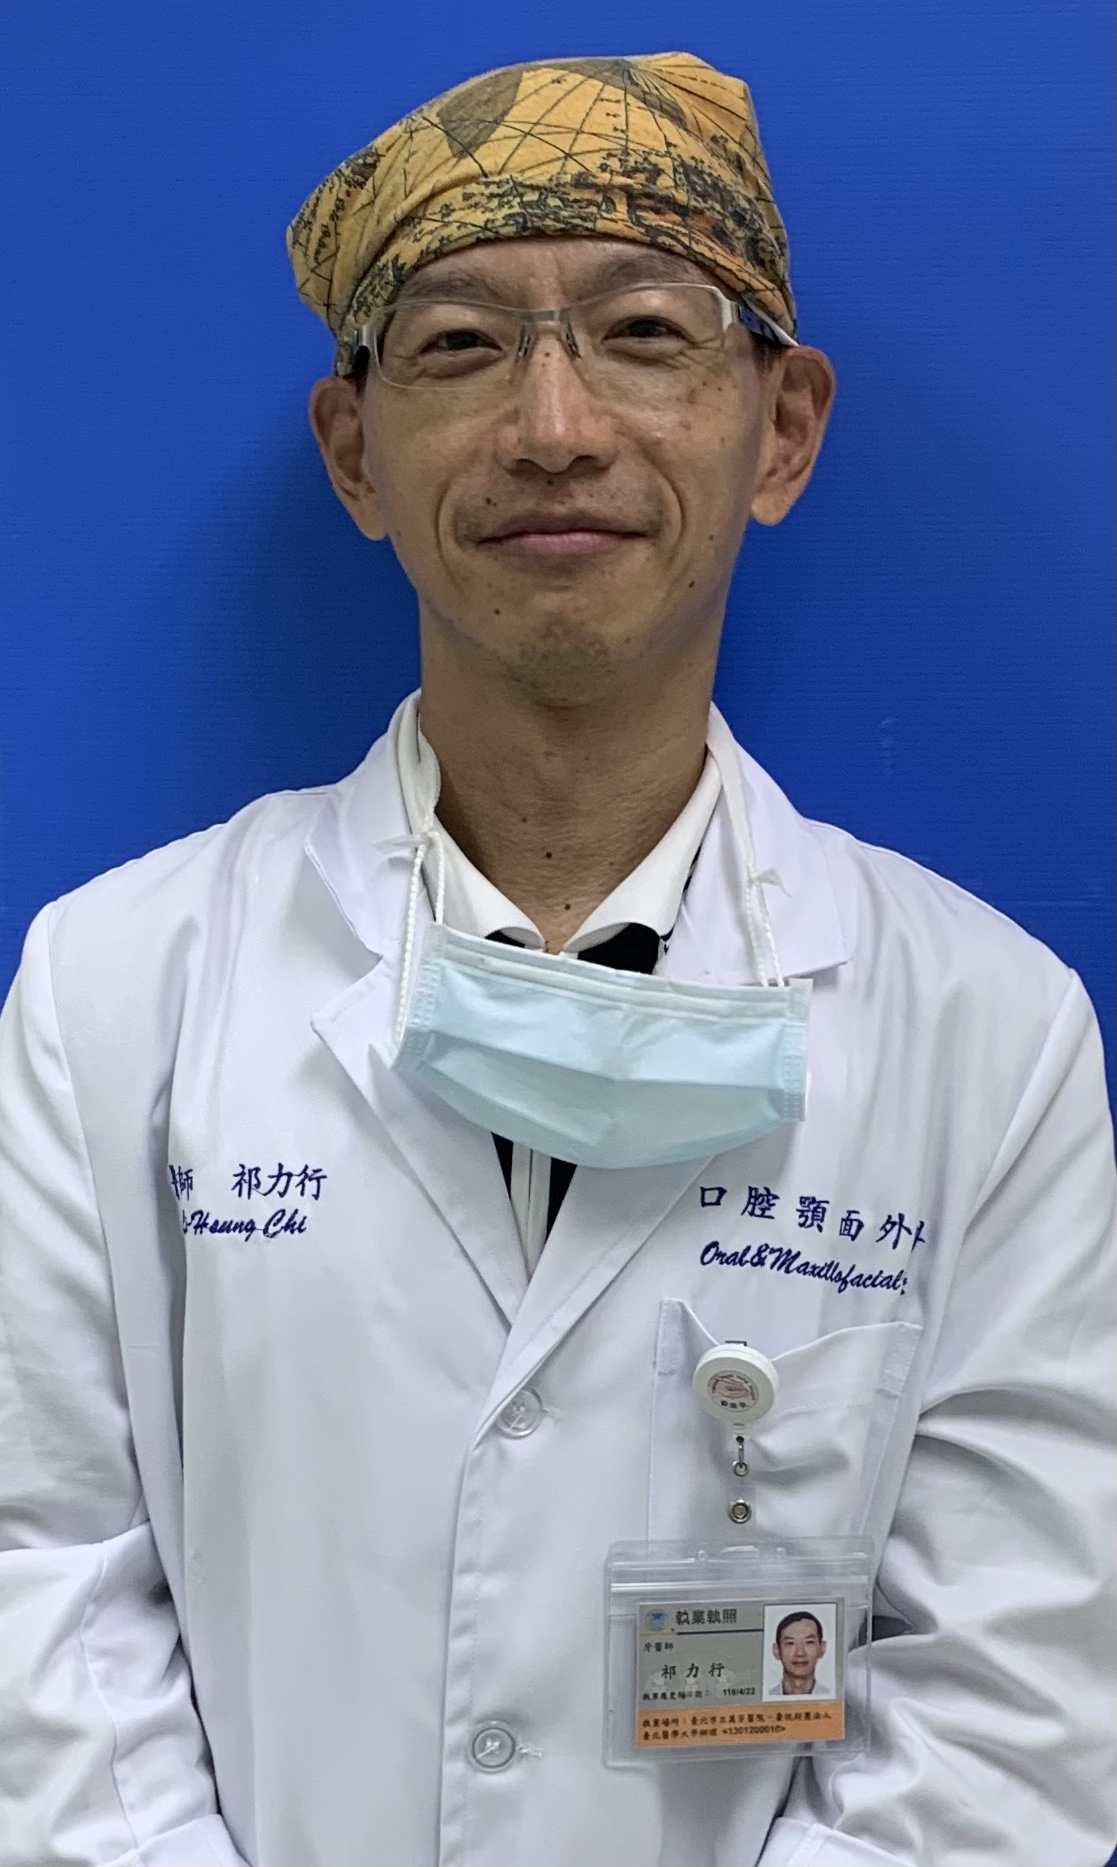
\includegraphics[height=40mm]{IMG_5507_Tex_portrait_TMWH.jpg}
\end{wrapfigure}

\noindent
Director (April 2021 - present)\\
Division of Oral and Maxillofacial Surgery, Department of Dentistry, Taipei Municipal Wanfang Hospital\\[4mm]
Attending physician (Jan. 2002 - present)\\
Division of Oral and Maxillofacial Surgery, Department of Dentistry,
Taipei Medical University Hospital\\
Taipei, Taiwan\\


% --- Start the two-column table storing the main content ---

% Set spacing between columns
\setlength{\tabcolsep}{8pt}

% Set the width of each column
\begin{longtable}{p{1.3in}p{4.8in}}

% --- Section: Research interests ---

\nohyphens{\color{OliveGreen}{Research interests}}
& Biostatistics with R/Python/C++ for survival analyses and deep learning, biomedical informatics; cancer research in vitro and in vivo; mindfulness meditation, laser acupuncture; forensic medicine. \\
& \\

% --- Section: Education ---
% my dissertation:
%1. Chi L-H. Global Transcriptomics and Proteomics Analyses for Biomarker Identification and Validation in Head and Neck Squamous Cell Carcinoma. Published online 2022/01/22.

\color{OliveGreen}{Education} 
& \textbf{Taipei Medical University and Academia Sinica} \hfill Taipei, Taiwan \\ 
& The Ph.D. Program for  Translational Medicine \hfill Feb. 2013 -- Feb. 2022 \\
& Mentors: Professors Yu-Chuan (Jack) Li, Michael Hsiao, Alex T.H Wu. \\
& \\

& \textbf{Taipei Medical University} \hfill Taipei, Taiwan \\
& MS in Biomedical Informatics \hfill Sep. 2011 -- Jan. 2013\\
& Mentor: Professor Yu-Chuan (Jack) Li.\\ % {\it GPA: X.YZ.}\\
& \\
% Yu-Chuan Jack Li M.D., Ph.D., FACMI

& \textbf{Taipei Medical University} \hfill Taipei, Taiwan \\
& BS in Dentistry \hfill Sep. 1988 -- Jun. 1994 \\
& \\% Mentors: Professors E, F. {\it GPA: X.YZ.}\\
& \\

% --- Uncomment the next few lines if you want to include some courses ---
%& \textbf{Selected coursework}
%\begin{itemize}[noitemsep,leftmargin=*]
%\item \underline{Relevant subject 1}: Course 1, Course 2, Course 3, Course 4
%\item \underline{Relevant subject 2}: Course 1, Course 2, Course 3, Course 4
%\end{itemize} \\

% --- Section: Awards, scholarships, etc. ---
% --- Note: section title is spread over two lines ---

{\color{OliveGreen}{Honors and award}} 
& Best Paper Presentation Award - 3rd Prize, at Translational Medicine
Program Retreat (Academia Sinica, Taiwan) \hfill 2017\\
%{\color{OliveGreen}{scholarships}} 
%& Name of award 2 (Organization that gave you the award)\hfill 2019 \\
%& Name of award 3 (Organization that gave you the award) \hfill 2018 \\
%& \\



% --- Section: Industry experience ---

%{\color{OliveGreen}{Industry experience}} 
%& {\textbf{Name of company,}} Division of company \hfill City, State\\
%& Title of job or internship \hfill Summer 2020 \\
%& Description of your responsibilities. Integer pretium semper justo. Proin risus. Nullam id quam. Nam neque. Phasellus at purus et lib ero lacinia dictum. Sed dolor lacus, imperdiet non, ornare non, commodo eu, neque.\\
%& \\
 
%& {\textbf{Name of company,}} Division of company \hfill City, State\\
%& Title of job or internship \hfill Summer 2020 \\
%& Description of your responsibilities. Integer pretium semper justo. Proin risus. Nullam id quam. Nam neque. Phasellus at purus et lib ero lacinia dictum. Sed dolor lacus, imperdiet non, ornare non, commodo eu, neque.\\
%& \\

% --- Section: Talks and tutorials ---

{\color{OliveGreen}{Presentation}} 
& \textbf{A Transcriptomic Analysis of Head and Neck Squamous Cell Carcinomas for Prognostic Indications} \hfill Sep. 10, 2021 \\
& The 8th Annual Academic Achievements Presentation of Translation Medicine Degree Program \\
& \\

& \textbf{Global Proteomics-based Identification
and Validation of Thymosin Beta-4 X-Linked as a Prognostic Marker for Head
and Neck Squamous Cell Carcinoma} \hfill Sep. 6, 2017 \\
& The 4th Translational Medicine
Program Retreat, Taipei, Taiwan. \\
& \\

& \textbf{Silencing JARID1B Suppresses
Oncogenicity, Stemness and Increases Radiation Sensitivity in Head and
Neck Squamous Cell Carcinoma} \hfill Sep. 4, 2015 \\
& The 2nd Annual Retreat of the
Translational Medicine Degree Program, Kaohsiung, Taiwan. \\
& \\


& \textbf{Glucose Transporter 4, encoded by gene
SLC2A4, as a Prognostic Marker for Head and Neck Squamous Cell
Carcinoma} \hfill Sep. 19, 2014 \\
& The 1st Annual Retreat of the Translational Medicine Degree Program, Taipei, Taiwan. \\
& \\


& \textbf{A Summary of International Partnership for Health Informatics Education} \hfill  2012 \\
& IPHIE2012 Master
class training of Health Informatics, University Of Minnesota, Twin
Cities, MN, U.S.A. \\
& \\

& \textbf{Recurrent Ameloblastic Carcinoma ex
Ameloblastoma of Maxilla - A case report} \hfill June 2005 \\
& ICOMS – 17th International
Conference on Oral and Maxillofacial Surgery, Vienna, Austria. \\
& \\



% --- Section: Various skills (programming, software, languages, etc.) ---

{\color{OliveGreen}{Skills}} 
& \textbf{Programming}\\
& Proficient in: R, Python/PyTorch. \\
& Familiar with: Matlab, SAS, C++. \\
& \\

& \textbf{Languages} \\
& Chinese, English (fluent) \\
& \\

% --- Section: Service and outreach ---

\color{OliveGreen}{Service and outreach by TMU} % Africa
& \textbf{Royal Health Mission in the Kingdom of Eswatini, southern Africa} \hfill Sep. 2014 -- Sep. 2019 \\
& attending physician working at the Manzana Clinic. \\
& \\

& \textbf{Missão Médica de Taiwan em São Tomé e Príncipe, west Africa} \hfill Nov. 2010 -- Jan. 2012 \\
& attending physician working at hospital central em São Tomé e Príncipe. \\
& \\

& \textbf{Taiwan Medical Mission in the Kingdom of Swaziland, southern Africa} \hfill May 2009 -- Nov. 2010 \\
& attending physician working at the Mbabane Government Hospital. \\
& \\

% --- Section: Professional society memberships ---
% --- Note: section title is spread over two lines ---

\nohyphens{\color{OliveGreen}{Professional memberships}}
& {\textbf{Taiwanese Association of Oral and Maxillofacial Surgeons (TAOMS)}} \hfill Jan. 2002 -- Present \\
%{\color{OliveGreen}{memberships}} 
& Taiwan Society of Forensic Medicine (TSFM) \hfill 2022-\\ 
& Taiwan Biophysics Society \hfill 2014-\\ 
& Taiwan Society for Integration of Chinese and Western Medicine (CWM) \hfill 2019-\\
& Chinese Medical Association of Acupuncture (CMAA, Taiwan) \hfill 2019- \\
& \\

% --- Section: Other interests/hobbies ---

%\nohyphens{\color{OliveGreen}{Manuscript under review}}
%& \textbf{A Global Genome-Wide Scan with Optimal Cutoff Mining for Emerging Biomarkers in Head and Neck Squamous Cell Carcinoma} \\
%& Chi, Li-Hsing and Wu, Alexander T H and Hsiao, Michael and Li, Yu-Chuan Jack.\\
%& \textit{Research Square [Preprint Server], 2020}\\
%& \\

%\pagebreak

\nohyphens{\color{OliveGreen}{References}} 
& Dr. Bou-yue Pemg, D.D.S., M.S.\\
& Director\\
%Attending physician and specialist,
& Oral and Maxillofacial Surgery, Department of Dentistry,
Taipei Medical University Hospital,
Taipei, Taiwan\\
& E-mail: pemg@tmu.edu.tw\\[0.5cm]


& Professor Yu-Chuan Jack Li, M.D.,  Ph.D.\\
& Professor\\
& Professional Master Program for Artificial Intelligence in Medicine, Taipei Medical University,
Taipei, Taiwan\\
& E-mail: jack@tmu.edu.tw\\[0.5cm]


& Professor Michael Hsiao, D.V.M., Ph.D.\\
& Research Fellow\\
& Genomics Research Center, 
Academia Sinica, Taipei, Taiwan\\
& E-mail: mhsiao@gate.sinica.edu.tw\\[0.5cm]

& Dr. Alex T.H Wu, Ph.D.\\
& Associate Professor\\
& Graduate Program in Translational Medicine,
College of Medical Science and Technology,
Taipei Medical University,
Taipei, Taiwan\\
& E-mail: chaw1211@tmu.edu.tw\\




\end{longtable}


% --- Section: Publications ---
\nohyphens{\color{OliveGreen}{Publications}} 
\printbibliography[heading=none] %, 
%\printbibliography[heading=subbibliography, notkeyword=donotinclude]

%\bibliography{Tex_publications_since2002.bib} % lib.bib file inside ref folder
%\bibliographystyle{model1-num-names}
% model1-num-names
% apacite
\nocite{*}

% --- End of CV! ---
\end{document}
%%%%%%%%%%%%%%%%%%%%%%%%%%%
% --- Section: Teaching experience, holistic ---

{\color{OliveGreen}{Teaching experience}} 
& \textbf{Teaching assistant, Department of Subject (University)} \hfill Fall 2020 \\
& STAT 123: Name of course here \\
& Topics and description of your responsibilities. Aliquam volutpat est vel massa. Sed dolor lacus, imperdiet non, ornare non, commodo eu, neque. \\
& \textit{Average student rating: X/5.} \\
& \\

& \textbf{Teaching assistant, Department of Subject (University)} \hfill Spring 2020 \\
& STAT 234: Name of course here \\
& Topics and description of your responsibilities. Aliquam volutpat est vel massa. Sed dolor lacus, imperdiet non, ornare non, commodo eu, neque. \\
& \textit{Average student rating: X/5.} \\
& \\

& \textbf{Teaching assistant, Department of Subject (University)} \hfill Spring 2020 \\
& STAT 345: Name of course here \\
& Topics and description of your responsibilities. Aliquam volutpat est vel massa. \\
& \textit{Average student rating: X/5.} \\
& \\








% --- Section: Research experience ---

\nohyphens{\color{OliveGreen}{Research experience}} 



& \textbf{ Title of project or lab where research was conducted} \\
& Mentors: Professor A (University) \hfill Month Year -- Present \\
& Description of your work. Summary of findings available \href{https://en.wikibooks.org/wiki/LaTeX/Hyperlinks}{here}. Sed dolor lacus, imperdiet non, ornare non, commodo eu, neque. Integer pretium semper justo. \\
& \\

& \textbf{Title of project or lab where research was conducted} \\
& Mentors: Professor B (University) \hfill Month Year -- Present \\
& This description of your work might spill onto the next page, which is fine. \hfill $\rightarrow$ \\
& Aliquam volutpat est vel massa. Sed dolor lacus, imperdiet non, ornare non, commodo eu, neque. Integer pretium semper justo. Proin risus. \\
& \\
